We investigated three versions of the AWP design described in the last section of the previous chapter. The first type we present is based on 3D printed \ce{Al2O3}, the second type is produced using ordinary 3D printed polymers and the third type consists of SLE fused silica glass waveplates as described in the previous chapter. The results are obtained through the minimization of the two objective functions defined in the previous chapter.

% This AWP type differs from the other two in the sense that the phase shift is not caused by form birefringence, but instead by intrinsic birefringence which stems from the crystallographic orientation of the material. The second type is similar to the fused silica glass AWP in the sense that it is also based on form birefringence but the structure is 3D printed by typical of the birefringence is not from the structure but instead on the crystallographic orientation of the material. 

\section{Ceramic}
In a publication by Ornik et al. it was shown that \ce{Al2O3} as a 3D printed ceramic exhibited birefringent properties. A birefringence of approximately $0.05$ was reported.  This value is fairly low compared to the birefringence of sapphire which is the crystalline form of \ce{Al2O3} and is known to have a birefringence of approximately $0.32$ \cite{Ornik2021}.  

\begin{figure}[h]
    \centering
    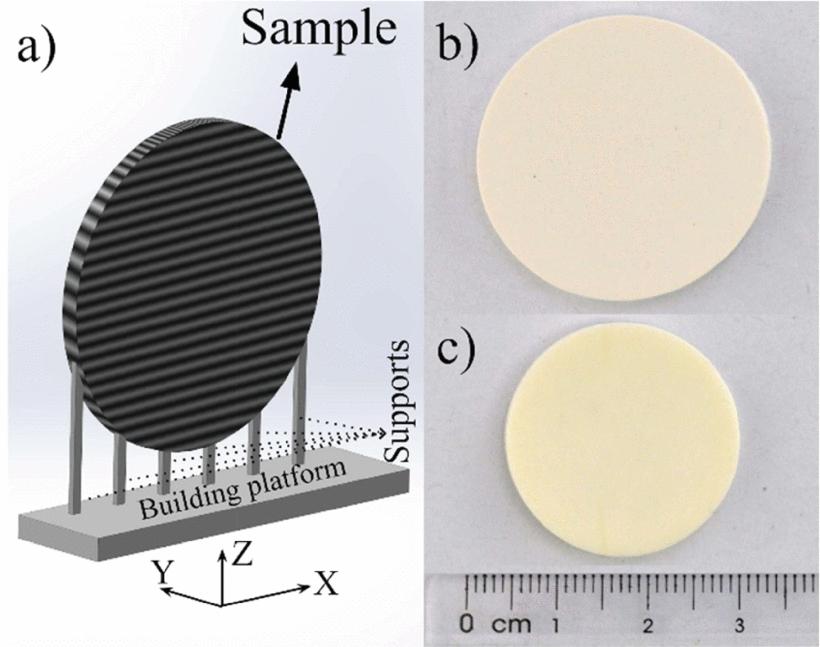
\includegraphics[scale=0.4]{images/5_chapter05/ornik1abc-3047514-large.png}
    \caption{aaa. Source: \cite{Ornik2021}}
    \label{fig:my_label}
\end{figure}

It was further shown that the 
The ceramic AWP consists of individual 3D printed 


\subsection{Simulation}
\subsection{CST}
\subsection{Fabrication error}

\section{Polymer}

\section{Fused silica glass}




